\chapter{The quest for cell barcodes}
\label{ch:seq}
In the previous chapters, I showed how we modified the inDrop microfluidic framework to a) accomodate a \acrshort{smart-seq}/Drop-seq-like \acrshort{scrna-seq} and b) implement a novel \acrshort{dropatac} protocol. The normal course of action would now be to separate the fragments from the pooled libraries based on their cell barcode, and account for \acrshort{pcr} induced bias by counting \acrshortpl{umi} (figure \ref{fig:seq_cellmatrix}). However, while the bulk characteristics of the resulting datasets met our expectations, we were unable to retrieve cellulcar barcodes, making it impossible to demultiplex our single cell libraries. In this chapter, I will explain how we attempted to diagnose the problem in our libraries, its possible origins and how to solve it in the future.\pms

% One of the most widespread strategies employed in single cell omics is to "tag" a cell's biological material (usually nucleic acids) using an oligonucleotide barcode. After \acrfull{ngs} of the oligonucleotide barcode, the material's cell of origin can be identified. In some protocols, including ours, the barcode also includes a \acrlong{umi}, a random nucleotide sequence which identifies each individual barcode. The \acrshort{umi} can be used to absolutely quantify fragments even after \acrshort{pcr} amplification (figure \ref{fig:seq_cellmatrix}) .\pms

\begin{figure}[ht]
\centerfloat
\includegraphics[width=\textwidth]{./ims/seq_cellmatrix.png}
\caption[Library demultiplexing]{\textbf{Library demultiplexing.} Transcripts in a pooled single cell library can be demultiplexed by assigning them to a common cell of origin based on their cell barcode. Transcripts can be quantified by counting \acrshortpl{umi}.}
\label{fig:seq_cellmatrix}
\end{figure}

\section{Illumina Next-Generation Sequencing}
In recent years, the San Diego-based Illumina has dominated the sequencing market, operating at a de facto monopoly \citep{greenleaf2014}. The company's sequencing adapters have been used extensively in single cell omics, often being directly incorporated into published methods and protocols. Two advantages of Illumina sequencing are throughput and accuracy. A single fragment is clonally amplified to produce a fluorescent signal that can be used to call bases with high accuracy. However, quality drops progressively as the sequencing goes on due to cumulative errors. The read length of sequencing by synthesis is thus limited. A schematic overview of a \acrshort{dna} strand undergoing the different steps of Illumina sequencing is given in figure \ref{fig:seq_illuminasequencing}. For a more detailed overview of bridge amplification on a glass substrate and sequencing by synthesis chemistry, see \cite{fedurco2006} and \cite{harris2008}.\pms

\begin{figure}[ht]
	\centerfloat
	\includegraphics[width=\textwidth]{./ims/seq_illuminasequencing.png}
	\caption[Strand progression during Illumina sequencing]{\textbf{Strand progression during Illumina sequencing.} \textbf{(1)} The fragment's P5 and P7 regions hybridise to the flow cell surface. \textbf{(2)} Complementary strands are synthesized and the original library is washed away, leaving only the freshly synthesised complement. \textbf{(3, 4)} Bridge amplification occurs, amplifying the single \acrshort{dna} strand to a densely packed clonal cluster. The P5 region is then cleave, leaving only P7-bound strands to be sequenced. \textbf{(5)} After the sequencing primer attaches to the P5 end, \acrfull{sbs} occurs. The combined fluorescent signal of all strands in a clonal cluster is optically detected as a bright spot on the flow cell surface and computationally translated to a base call. \textbf{(6)} Each fragment's sample index is sequenced using an index primer. \textbf{(7, 8)} In paired-end sequencing, a second round of bridge amplification occurs. The P7 end is now cleaved, leaving P5-bound strands to be sequenced. Adapted from Harvard MGH Sequencing Core Resources.}
	\label{fig:seq_illuminasequencing}
\end{figure}

We sequence our \acrshort{scrna-seq} and \acrshort{scatac-seq} libraries differently from classical inDrop and Drop-seq libraries, which read their whole barcode sequence in a single go. Due to the split-pool \acrshort{pcr} reaction we use to barcode the hydrogels, both halves of the barcode are separated by a 32 \acrshort{bp} \acrshort{pcr} primer site. This primer site is used as a read primer site for both halves of the barcodes (figure \ref{fig:seq_nextseq_library}). By not reading the \acrshort{pcr} adapter inbetween both barcode halves, and using it as a read primer site instead, we increase the cycle budget for the \acrshort{cdna} by 32 cycles. The process illustrated in figure \ref{fig:seq_nextseq_library}a.\pms

\begin{figure}[ht]
\centerfloat
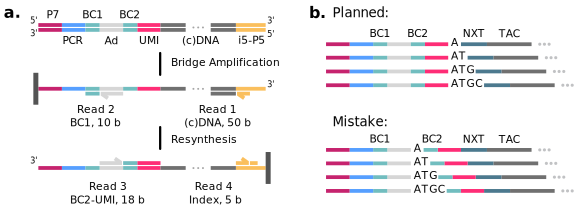
\includegraphics[width=\textwidth]{./ims/seq_nextseq_library.png}
\caption[Custom sequencing process and stagger sequence]{\textbf{Custom sequencing process and stagger sequence.} \textbf{a.} After the library is bridge-amplified, the first two reads will read the 3' \acrshort{cdna} (\acrshort{rna-seq} libraries) or \acrshort{dna} (\acrshort{atac-seq} libraries) fragment and the first half of the barcode. The reverse complement is then synthesized, and the second half of the barcode and index are read by read 3 and 4. \textbf{b.} Incorrect placement of stagger sequence in \acrshort{dropatac} library.}
\label{fig:seq_nextseq_library}
\end{figure}

The \acrshort{dropatac} library has a similar structure to the inDrop library, but also has a staggered barcode sequence due to mistake in the barcode design (figure \ref{fig:seq_nextseq_library}b). This stagger sequence was originally intended to be located after the \acrshort{umi}, right before the Nextera Tn5 adapter sequence. Such a stagger would shift the Tn5 adapter by one nucleotide and, enabling us to extend the read cycles beyond BC2 without risking low base-call accuracy associated with highly similar sequences. Paired-end reads would allow us to map the exact length of the fragments. By mistake however, the stagger sequence was placed before BC2 instead, complicating the barcode identification process by requiring a slight change to the whitelist for barcode 2.\pms

\clearpage
\begin{wrapfigure}{L}{\textwidth/2}
\centering
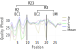
\includegraphics[width=\textwidth/2]{./ims/seq_ind_qual.png}
\captionsetup{margin={6pt,6pt},labelfont=bf}
\caption[inDrop barcode read quality]{\textbf{inDrop barcode read quality.}}
\label{fig:seq_ind_qual}
\vspace{-20pt}
\end{wrapfigure}

The sequencing data was mapped to the reference genome and examined. As mentioned in chapters \ref{ch:indrop} and \ref{ch:dropatac}, the bulk properties of the library were satisfactory, but we could not cell-demultiplex the transcripts. The quality of the barcode reads (Read 2 and Read 3, which are in-silico concatenated to a single virtual read, referred to as R23) was low and inconsistent compared to the \acrshort{cdna} reads (figure \ref{fig:seq_ind_qual}). Only 723 combined R23 reads had a mean Phred quality of > 34 (corresponding to a 99.96\% average base call certainty), and out of these 723 reads, only 2 matched our barcode whitelist. Unfiltered, less than 0.01\% of the R23 reads matched the 384 x 384 barcode whitelist completely. When looking at R2 and R3 individually, 3\% and 10.9\% of reads matched the whitelist respectively. The vast majority of R23 contained poly-G noise, illustrated in figure \ref{fig:seq_bcdist}.\pms

Similarly to the inDrop library, our single cell \acrshort{dropatac} library could not be cell-demultiplexed. The problem is even worse - less than 1\% of all R23 carry even one whitelisted half-barcode. We did not observe poly-G, but the single cell library's BC2 showed a high percentage of A bases. Even in the "bulk" \acrshort{dropatac} library, which is produced using a single dissolved barcoded primer in all droplets, no significant amount of barcodes was found. Here, we would expect the single barcode used in the experiment to dominate the distribution - but it did not.\pms

We briefly attempted to apply the \acrfull{blat} algorithm to R23 to see if we could retrieve any reads that resembled a whitelisted barcode (within 2 Hamming distance). However, due to the large database of 147k whitelisted barcodes, the algorithm was inefficient. We therefore tried to use \verb|blat| on R2 and R3 separately - where we had to match only 384 whitelisted barcodes per read - but found no significant number of hits. We later on discovered that the \acrshort{blat} algorithm is ill-suited for matching sequences of 25 \acrshort{bp} or fewer, which at least partially explains the output we had achieved. In section \ref{sec:seq_minion}, we use the \verb|cutadapt| algorithm to look at a MinION sequencing dataset, a different algorithm which could be used to extract more information out of the "failed" inDrop dataset in the future.\pms

\begin{figure}[ht]
\centerfloat
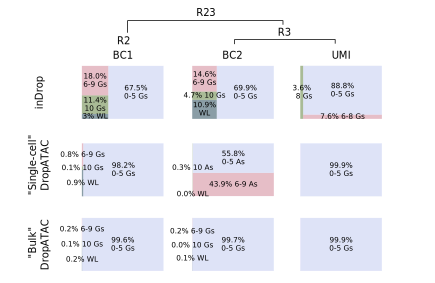
\includegraphics[width=\textwidth]{./ims/seq_ind_bcdist.png}
\caption[Barcode whitelist percentages]{\textbf{Barcode whitelist percentages.} R2 and R3 refer to Read 2 and Read 3, R23 to the in-silico concatenation of the two. WL refers to the percentage of reads that could be retrieved from the whitelist, and 10Gs, 6-9Gs and 0-5Gs denote the number of Gs in the non-whitelisted read.}
\label{fig:seq_bcdist}
\end{figure}

We highly suspect that the Illumina sequencing process itself may have failed, and not our inDrop/Drop-ATAC protocols. The split-pool barcoding process, should not generate, under any circumstances, the poly-G or random sequence barcodes that are read. During the second isothermal amplification step, the second barcode half carrying the poly-T tail can only be appended to the bead primer if a BC1 was was appended there prior. If the primer released by the bead has no poly-T, it cannot capture a poly-A\textsuperscript{+} \acrshort{mrna} fragment. It is therefore unlikely, especially at the scale we observe, that partial or incorrectly synthesised barcoded primers on the \acrshortpl{bhb} led to the effects we observe here.\pms

\begin{wrapfigure}{L}{\textwidth/3}
\centering
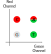
\includegraphics[width=\textwidth/3]{./ims/seq_2channel.png}
\captionsetup{margin={6pt,6pt},labelfont=bf}
\caption[Illumina 2 channel technology]{\textbf{Illumina 2 channel technology.}}
\vspace{-20pt}
\label{fig:seq_2channel}
\end{wrapfigure}

Since the \acrshort{cdna} read (R1) and the sample index read (R4), which both use standard Illumina sequencing primers, were sequenced fine, our prime suspect became the custom sequencing primers used to read both barcode halves (R2 and R3). In our experiments, we used the Illumina NextSeq 500 platform, which uses a 2-dye colour system to identify the four different bases (figure \ref{fig:seq_2channel}). Poly-G reads, which are indistinguishable from \textit{no signal} on the NextSeq 500 platform (figure \ref{fig:seq_2channel}), are most likely caused by the custom sequencing primer not hybridising. When this happens, \acrlong{sbs} cannot occur, and the base calling software will interpret the lack of signal as a G nucleotide. Inversely, the non-whitelisted, non-poly-G reads could be explained by the custom sequencing primer hybridising where we do not expect it. However, we extensively searched through the theoretical fragment produced by our protocol and did not find any (close) match, and at a length of 32 base, it is unlikely to hybridise to the \acrshort{cdna}.\pms

Finally, it is also possible that this NextSeq 500 run in particular yielded bad results due to technical failure. The low-quality of some reads can be attributed to overclustering. Our sequencing run had a cluster density of \SI{312 000}{\per\mm\squared} and a filter pass rate of 61.5\%, far beyond the flow cell's recommended \SI{200 000}{\per\mm\squared}. When overclustering occurs, base calling becomes less precise due to overlap in signals from different clusters.\pms

% Due to the high 3' enrichment of our library, we also know that the fragments that our protocol produces are the barcoded 3' ends. In theory, an event could occur where a throughout the library preparation, remnants of the

% Moreover, short sequences are filtered out during the multiple Ampure bead purification steps we perform during library preparation. and due to the many (labour-intensive) washing steps following synthesis, it is highly unlikely that any pa

The indications above prompted us to take the following course of action:
\begin{enumerate}
\item Sequence a number of inDrop and \acrshort{dropatac} fragments by classical Sanger sequencing. Sanger sequencing can process the whole library fragment in one read, and does not rely on our custom sequencing primers. It therefore provides the true sequence of a low number of purified fragments, but cannot give us insights in macro-scale qualities of the sequencing libraries.
\item Re-sequence the libraries on the NextSeq 500 to eliminate technical failure, this time using a reduced concentration of input \acrshort{dna} and an increased percentage of spiked-in PhiX. PhiX is an Illumina spike-in standard that can be used as a control for sequencing accuracy and clustering efficiency.
\item Produce a new batch of \acrshortpl{bhb} that do not require custom sequencing primers, perform a new custom inDrop run and sequence on the NextSeq 500.
\item Sequence the library on the Oxford Nanopore Minion. This platform is also capable of sequencing the library's complete fragment length, but at a much larger scale than Sanger sequencing. Since it is a single-molecule sequencing technology, it does suffer from low single-base accuracy.
\end{enumerate}

\section{Sanger Sequencing}
In order to sequence a small number of fragments with high fidelity, we reached back for the gold standard approach: Sanger sequencing. To amplify the fragments, which have a mean length of 400 bp, we used TOPO cloning followed by \acrshort{dna} purification. We sequenced 9 fragments from the inDrop library, 5 from the single cell \acrshort{dropatac} library and 10 from the two "bulk" \acrshort{dropatac} libraries.\pms

The results are illustrated in figure \ref{fig:seq_sanger}. The Sanger sequencing showed that 4 out of the 9 sampled inDrop fragments perfectly matched the theoretical fragment we envisioned. The other fragments had a number of minor defects, but in total 15 of the 18 half-barcodes sequenced matched the whitelist. The \acrshort{dropatac} fragments showed similar characteristics. Out of the 10 "bulk" \acrshort{dropatac} fragments, 9 carried the barcode combination used in the experiment. The single cell \acrshort{dropatac} library also had 5/5 fully whitelisted barcodes. One of the fragments did not contain a captured \acrshort{dna} fragment. It is unclear how this happened during the library preparation, and how it escaped the Ampure short-fragment filtering.\pms

\begin{figure}[ht]
\centerfloat
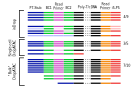
\includegraphics[width=\textwidth]{./ims/seq_sanger.png}
\caption[Sanger sequencing results]{\textbf{Sanger sequencing results.} Lighter colour denotes slight deviation from the expected sequence. The bottom inDrop fragment was inverted in the TOPO cloning, leading to a barcode at the utmost end of the Sanger sequencing run, leading to low base-calling accuracy.}
\label{fig:seq_sanger}
\end{figure}

The Sanger sequencing confirmed our suspicions that the Illumina sequencing run was not representative of the true library. While the library had a number of true defects, the majority of sequenced fragments had a whitelisted barcode and an intact read primer site. Theoretically, it is possible that these well-behaved fragments were picked by chance, but given that TOPO cloning can be assumed to be unbiased, it's unlikely that our library is not enriched with the good fragments detected here. We could thus narrow the problem down to flawed sequencing, most likely associated with our custom read primers.\pms

\section{NextSeq 500 Re-sequencing}

% \begin{wrapfigure}{L}{\textwidth/3}
% \centering
% 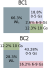
\includegraphics[width=\textwidth/3]{./ims/seq_ind_reseq_bcdist.png}
% \captionsetup{margin={6pt,6pt},labelfont=bf}
% \caption[Barcode whitelist percentage]{\textbf{Barcode whitelist percentage.}}
% \label{fig:seq_ind_reseq_bcdist}
% \vspace{-30pt}
% \end{wrapfigure}

We re-sequenced the inDrop and single cell \acrshort{dropatac} libraries on the NextSeq 500 to eliminate the possibility of technical failure during the first run. This time, the spiked-in PhiX fraction was strongly increased from 1\% to 20\% and the amount of input \acrshort{dna} was reduced. These factors led to a lower clustering density of \SI{205 000}{\per\mm\squared} with 83.1\% of clusters passing filtration - marginally overclustered, but not alarming. The overall sequencing quality of the re-sequencing run was better than the first run. Compared to the first sequencing run, the mapping percentages remained the same for both inDrop (56\%) and \acrshort{dropatac} (77\%). Figure \ref{fig:seq_reseq_igv} shows the gene coverage of the re-sequencing run, which was also near-identical to the first sequencing run.\pms

In the inDrop library, we still found poly-G reads, but not to the extent of the first sequencing run. The quality of the inDrop barcode reads also improved to 66\% of the BC1 reads and 28.3\% of the BC2 reads matching to entries in their respective 384 barcode whitelist (figure \ref{fig:seq_reseq_bcdist}). Since both halves are needed for a full barcode, the number of full barcodes is lower - 23.6\% of the BC1 + BC2 combinations matched the master whitelist of 384 x 384 combinations.\pms

\begin{figure}[ht]
\centerfloat
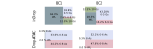
\includegraphics[width=\textwidth]{./ims/seq_reseq_bcdist.png}
\caption[Re-sequencing run inDrop and Drop-ATAC barcode distribution]{\textbf{Re-sequencing run inDrop and Drop-ATAC barcode distribution.} The original inDrop and single cell \acrshort{dropatac} libraries were re-sequenced on the NextSeq 500, but at reduced clustering density. The inDrop library showed a strongly improved fraction of reads mapping to the barcode whitelist, but the \acrshort{dropatac} library did not.}
\label{fig:seq_reseq_bcdist}
\end{figure}

As for the \acrshort{dropatac} library, the new sequencing data did not provide any more information. In fact, whereas only the second barcode half had a poly-A problem in the first sequencing run, both halves showed poly-A reads in the second sequencing run. In a sense, the poly-A problem can be seen as the inverse of the poly-G problem, as A is encoded by the combination of red and green signal on the NextSeq platform (figure \ref{fig:seq_2channel}). As of now, we have no explanation for the poly-A reads, given that they are not "true" reads as indicated by the Sanger sequencing, and that they were not present in the first sequencing run of the same library. At any rate, so far, we have been unsuccessful in retrieving barcodes from the \acrshort{dropatac} system due to the sequencing errors we experienced. The logical next step is to re-synthesize the \acrshort{bhb} barcodes using Illumina's TruSeq adapters instead of our custom read primers. Such a preliminary trial was performed for the inDrop library, and will be discussed in the following section.\pms

% \begin{wrapfigure}{R}{\textwidth/3}
% \centering
% 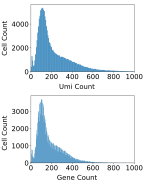
\includegraphics[width=\textwidth/3]{./ims/seq_reseq_distribution.png}
% \captionsetup{margin={6pt,6pt},labelfont=bf}
% \caption[Gene and UMI counts]{\textbf{Gene and UMI counts}}
% \label{fig:seq_ind_reseq_distribution}
% \vspace{-30pt}
% \end{wrapfigure}

As mentioned in chapter \ref{ch:indrop}, we systematically overloaded the inDrop run with cells to ensure an \acrshort{rna-seq} signal was present during the library preparation stages. This approach leads to severe undersequencing of the single cell transcriptomes. The number of cells with more than 1000 \acrshort{umi} counts (corresponding to 1000 unique transcripts captured) is only 699, and only 283 cells detected more than 750 genes. The mean number of \acrshortpl{umi} was 222, and the mean number of genes detected was 158. These metrics are low compared to what can be expected from a 10x Chromium \acrshort{scrna-seq} run (figure \ref{fig:seq_compar_ngene_numi}), but should improve when the sequencing depth per cell is increased. The general approach for selecting cells for further analysis is to find a steep drop in \acrshort{umi} count in the barcode rank plot (figure \ref{fig:seq_ind_kneeplot}). This sharp drop indicates the transition from true cells to noise associated with barcodes released into droplets without cells. In our dataset, no such steep drop was observed until the very end, which indicates that there is a gradual decline in \acrshort{umi} count. We can again explain this phenomenon by the cell overloading. Clearly, cell loading needs to go down in the future to increase per-cell sequencing depth.\pms

\begin{figure}[ht]
\centerfloat
\includegraphics[width=\textwidth]{./ims/seq_ngenenumicompar.png}
\caption[Gene and UMI count comparison]{\textbf{Gene and UMI count comparison.} Our method underperformed on the single cell level compared to Drop-seq and 10x Chromium \acrshort{scrna-seq}.}
\label{fig:seq_compar_ngene_numi}
\end{figure}

\begin{figure}[ht]
\centerfloat
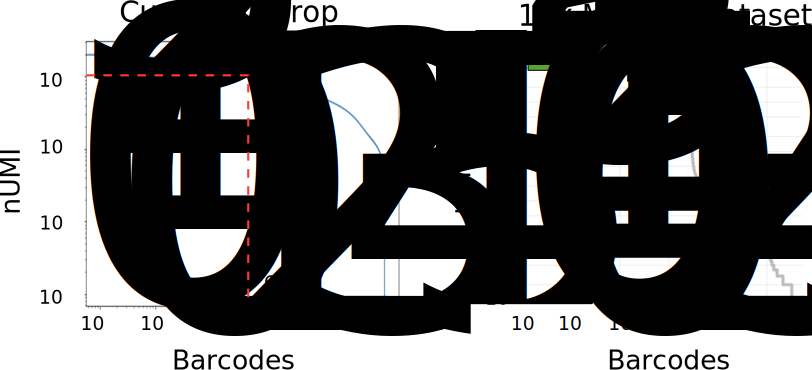
\includegraphics[width=\textwidth]{./ims/seq_kneeplot.png}
\caption[Barcode rank plots]{\textbf{Barcode rank plots.} Barcodes are ranked by the number of \acrshortpl{umi} they were associated with in the dataset. The steep decline in the 10x Chromium MM087 dataset indicates the transition from "true" cells to droplets containing only a barcoded hydrogel bead, and no cell.}
\label{fig:seq_ind_kneeplot}
\end{figure}

We were interested to see if the new inDrop library showed any resemblance to previous \acrshort{scrna-seq} datasets from the same MM087 cell line. We therefore performed \acrfull{cca} on the 699 inDrop cells that had a \acrshort{umi} count of > 1k combined with MM087 Drop-seq data and 10x Chromium \acrshort{scrna-seq} data from several MM cell lines (figure \ref{fig:seq_cca}). The Seurat \acrshort{cca} algorithm attempts to find shared sources of variation in gene expression (canonical correlation) between the different samples. The canonical components that explain most variation in the data are selected and further "aligned" (normalised) so they can be directly compared. The dimension-reduced correlation is then visualised using \acrfull{tsne}, which further reduces the aligned canonical correlation components until two dimensions remain, which can be plotted. The resulting plot shows a systematic clustering of cells that share common sources of variation. We hypothesized that our MM087 \acrshort{scrna-seq} dataset would cluster together with the 10x and Drop-seq datasets of the same cell line, but not with the other cell lines. In essence, this would mean that the datasets from the three techniques yield the same information. As is evident in the graph, this was not the case. Our cells mixed together with the Drop-seq dataset in the middle of the plot. This indicates that the inDrop and Drop-seq data did not contain enough information to be co-clustered with the 10x MM087 dataset. The lack of information is also evident in figure \ref{fig:seq_compar_ngene_numi}.\pms

\begin{figure}[ht]
\centerfloat
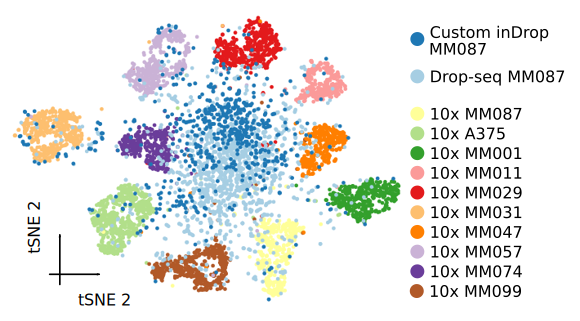
\includegraphics[width=\textwidth]{./ims/seq_cca.png}
\caption[MM087 canonical correlation analysis]{\textbf{MM087 canonical correlation analysis.} Our custom inDrop dataset does not co-cluster with the 10x Chromium MM087 dataset.}
\label{fig:seq_cca}
\end{figure}

We then briefly assessed the bulk properties of the re-sequenced library. We took all the datasets used in the previous analysis and removed the cell identifiers, transforming them from single cell datasets to bulk datasets. We then performed a regular correlation analysis between all the datasets and found that the inDrop dataset was in in fact significantly more correlated with the 10x MM087 dataset (p < 0.01, figure \ref{fig:supp_seq_ind_reseq_corr}).\pms

% \begin{wrapfigure}{R}{\textwidth/3}
% \centering
% 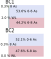
\includegraphics[width=\textwidth/3]{./ims/seq_dat_reseq_bcdist.png}
% \captionsetup{margin={6pt,6pt},labelfont=bf}
% \caption[Barcode whitelist percentage]{\textbf{DropATAC re-sequence barcode whitelist percentage.}}
% \label{fig:}
% \end{wrapfigure}

\clearpage
\section{Reduced Complexity inDrop Repetition}

\begin{wrapfigure}{L}{\textwidth/3}
\centering
\includegraphics[width=\textwidth/3]{./ims/seq_ind4_bcdist.png}
\captionsetup{margin={6pt,6pt},labelfont=bf}
\caption[4 x 4 inDrop library barcode distribution.]{\textbf{4 x 4 inDrop library barcode distribution.}}
\label{fig:seq_ind4_bcdist}
\vspace{-20pt}
\end{wrapfigure}

The entire process of producing and barcoding hydrogel, and using them in the custom inDrop protocol was repeated on MM074 cells. This time, we replaced the adapter sequence between both barcode halves with Illumina's standard TruSeq read primer sequence, allowing us to sequence the barcodes using well-defined and tested read primers. In order to save time and cost, only 4 x 4 different barcode combinations were used. The new 4 x 4 library was sequenced together with the previous 384 x 384 library on the same NextSeq 500 run and shared many of its improved sequencing properties. We were able to match a higher number of barcode reads to their respective whitelist, but there was again a high number of pure G-reads. We did not explore the single cell properties of this library since it would only be able to separate 16 virtual "cells".\pms

The reduced complexity inDrop run, together with the Sanger sequencing, confirmed our suspicions that many of the problems we encountered could be mitigated by using standard sequencing primers. Whereas the dual barcode read system was originally put in place to assign more sequencing cycles to the \acrshort{cdna}, we now realise that this approach causes more problems than it solves. In the current system, the fragment is re-sequenced after the first barcode half is read, and the second half of the barcode is read on the newly synthesized complement. Physically, the two strands that are being read are not the same, which manifests itself as a steep drop in quality between both reads. We are therefore thinking about a redesigned system with a shorter adapter sequence in-between both barcodes, allowing the barcode to be sequenced in a single read. The problem of the poly-G reads remains, and can most likely be reduced further, but never completely. Other single cell sequencing techniques also filter out a large portion of the reads. A last resort solution could be to use a 4-channel sequencing system such as the Illumina MiSeq. In this system, every base is encoded by its own fluorescence signal, meaning we could discern true G reads from an absence of signal.\pms

\newpage
\section{MinION Sequencing}
\label{sec:seq_minion}
% \begin{wrapfigure}{R}{\textwidth/2}
% \centering
% 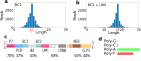
\includegraphics[width=\textwidth/2]{./ims/seq_minion.png}
% \captionsetup{margin={6pt,6pt},labelfont=bf}
% \caption[MinION sequencing barcode feature lengths distributions and fraction table]{\textbf{MinION sequencing barcode feature lengths distributions and fraction table.}}
% \label{fig:seq_minion}
% \vspace{-20pt}
% \end{wrapfigure}

The final measure we used to extract the last drop of information from the original 384 x 384 inDrop library was Oxford Nanopore MinION sequencing. The MinION sequencer works by pulling single \acrshort{dna} molecules through a nanopore and inferring base calling information from the change in electrical resistance over the pore. It can sequence long reads (up to 200 kbp), but with low single-base accuracy \citep{bowden2019}. We ran the MinION sequencer for 12 hours, during which the 1200 functional pores generated 276k reads which passed MinKNOW base-calling software's internal filter. The individual base quality is low - the mean read quality was 8.6, and from the 126 megabases read, only 17\% had a Phred quality score of > 10 (corresponding to a base call confidence of 90\%). A 1 in 10 chance for incorrect base calls is too low to attempt to match barcodes to the whitelist. Figure \ref{fig:seq_minion_qual} shows the average average quality and length of each read. The mean read length of 457 bp corresponds to what we expected from our library's electropherogram. The longer length band that separates from the rest of reads is most likely a remnant of a \acrshort{cheq-seq} library which was sequenced on the MinION device prior to our run. The MinION flow-cell can be reused multiple times, but will suffer from sample carry-over in doing so.\pms

\begin{figure}[ht]
\centerfloat
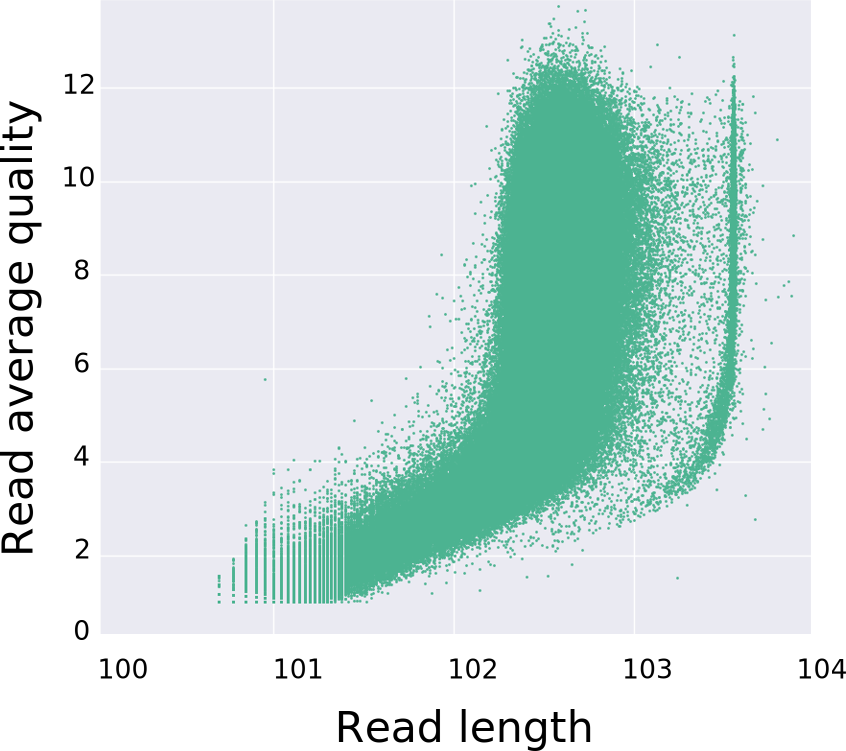
\includegraphics[width=\textwidth/3*2]{./ims/seq_minion_jasper.png}
\caption[MinION read length and quality]{\textbf{MinION read length and quality.} "Read average quality" denotes the average base calling quality of each single read, expressed as a Phred quality score.}
\label{fig:seq_minion_qual}
\end{figure}

Since Nanopore sequencing yields full length fragments, we had to extract the barcode locations ourselves. For this task, we used the \verb|cutadapt| adapter trimming tool \citep{martin2011}, which can (partially) match and find adapter sequences and manipulate the sequences attached to them. First, we removed all the reads that did not contain the bead primer sequence, which already eliminated 63\% of the reads. We then looked at only those reads that also contained the custom read site and the poly-T tail. All reads now contain the sequences that flank both barcode halves, meaning we could now look at the length of the barcodes. We found that there was a general adherence to the expected size, with 28\% of the BC1 sequences being exactly 10 bp, and 50\% of BC2 + \acrshort{umi} being exactly 18 bp in length, corresponding to the 10 bp barcode half and 8 bp \acrshort{umi} (figure \ref{fig:seq_minion}). The MinION sequencer is prone to both insertions and deletions, so some deviation is to be expected. We did not observe any such insertions or deletions in the Sanger sequencing data. We also observed that the minION sequencing did not yield any significant poly-G stretches, once again confirming that the poly-G reads produced by the NextSeq 500 were not true reads.\pms

\begin{figure}[ht]
\centerfloat
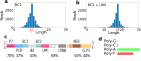
\includegraphics[width=\textwidth]{./ims/seq_minion.png}
\caption[MinION sequencing barcode feature lengths distributions]{\textbf{MinION sequencing barcode feature lengths distributions.} \textbf{(a, b)} Distribution of stretch between PCR site and Adapter (BC1) and between Adapter and Poly-T/A (BC2+\acrshort{umi}). \textbf{(c)} Idealised fragment, percentage indicates number of MinION reads that have that particular feature. \textbf{(d)} Fraction of fragments that have at least a single Poly-N sequence, defined as an uninterrupted stretch of 10 identical nucleotides.}
\label{fig:seq_minion}
\end{figure}
